\documentclass[12pt]{article}

%%%%%%%%%%%%%%%%%%%%%%%%%%%%%%%%%%%%%%%%%%%%%%%%%%%%%%%%%%%%%%%%%%%%%%%%
%                                                                      %
%               LATEX COMMANDS FOR DOCUMENT SETUP                      %
%                                                                      %
%%%%%%%%%%%%%%%%%%%%%%%%%%%%%%%%%%%%%%%%%%%%%%%%%%%%%%%%%%%%%%%%%%%%%%%%

%\usepackage{bookmark}
\usepackage[us,nodayofweek,12hr]{datetime}
\usepackage{graphicx}

\usepackage{tcolorbox}
\usepackage{fullpage}
\usepackage{graphicx}
\usepackage{tabularx}
\usepackage{multirow}
\usepackage{subfigure}
\usepackage{wrapfig}
\usepackage{textcomp}
\usepackage[square, comma, numbers, sort&compress]{natbib}
\usepackage[hang,small,bf]{caption}
\usepackage{parskip}
\usepackage[margin=1in,footskip=0.5in]{geometry}
\usepackage{amsmath}
\usepackage{mdwlist}
\usepackage{epstopdf}
\usepackage[section]{placeins}

\newcommand{\para}{\vspace{5mm} \noindent}
\newcommand{\parafig}{\vspace{4mm} \noindent}
\newcommand{\paraeq}{\vspace{1mm} \noindent}
\newcommand{\negparafig}{\vspace{-4mm} \noindent}
\newcommand{\negparaeq}{\vspace{-1mm} \noindent}

\addtolength{\parskip}{1\parskip}

\bibliographystyle{plain}
%\bibliographystyle{ieeetr}
%many other bibliography styles are available (IEEEtran, mla, etc.). Use one appropriate for your field.

\hyphenation{pre-par-ing} %add hyphenation rules for words TeX doesn't know

%\usepackage[square,comma,numbers,sort&compress]{natbib}
%\usepackage{hypernat}
% Other useful packages to try
\usepackage{amsmath}
\usepackage{amssymb}
\usepackage{accents}

\usepackage{setspace}
\usepackage{algorithm}
\usepackage{algorithmic}
%
% Different fonts to try (uncomment only fontenc and one font at a time)
% (you may need to install these first)
%\usepackage[T1]{fontenc} %enable fontenc package if using one of the fonts below
%\usepackage[adobe-utopia]{mathdesign}
%\usepackage{tgschola}
%\usepackage{tgbonum}
%\usepackage{tgpagella}
%\usepackage{tgtermes}
%\usepackage{fourier}
%\usepackage{fouriernc}
%\usepackage{kmath,kerkis}
%\usepackage{kpfonts}
%\usepackage[urw-garamond]{mathdesign}
%\usepackage[bitstream-charter]{mathdesign}
%\usepackage[sc]{mathpazo}
%\usepackage{mathptmx}
%\usepackage[varg]{txfonts}


%%%%%%%%%%%%%%%%%%%%%%%%%%%%%%%%%%%%%%%%%%%%%%%%%%%%%%%%%%%%%%%%%%%%%%%%
%                                                                      %
%        DOCUMENT SETUP AND INFORMATION FOR PRELIMINARY PAGES          %
%                                                                      %
%%%%%%%%%%%%%%%%%%%%%%%%%%%%%%%%%%%%%%%%%%%%%%%%%%%%%%%%%%%%%%%%%%%%%%%%

\begin{document}

%%%%%%%%%%%%%%%%%%%%%%%%%%%%%%%%%%%%%%%%%%%%%%%%%%%%%%%%%%%%%%%%%%%%%%%%

\vspace{7cm}
\begin{center}
   {\bf\Large An Incremental Kinematics Implementation for Finite Element Applications in Finite Deformation Continuum Mechanics}
\end{center}

\vspace{1.5cm}
\begin{center} 
{\bf\large Omar Hafez, Brian Giffin, Sam Mish, Mark Rashid}\\

%\vspace{5mm}
{Department of Civil \& Environmental Engineering}\\
{University of California, Davis}\end{center}

\abstract{The use of hypoelastic material models for applications in finite deformation solid mechanics has led to the development of so-called ``incrementally objective'' algorithms, which provide a means of updating the state of stress in a material over successive increments of deformation. (Address shortcomings of current/older methods still in common use.) This paper presents a ``strongly objective'' stress update algorithm which relies upon an efficient eigendecomposition of the incremental stretch tensor to retain accuracy in evaluating finite element residual and consistent tangent contributions. The accuracy of the method is compared against other approaches commonly found in commercial finite element software, and its nonlinear convergence performance is examined when either exact or approximate tangent terms are utilized.}

%%%%%%%%%%%%%%%%%%%%%%%%%%%%%%%%%%%%%%%%%%%%%%%%%%%%%%%%%%%%%%%%%%%%%%%%

% Each chapter can be in its own file for easier editing and brought in with the \include command.
% Then use the \includeonly command to speed compilation when working on a particular chapter.
%%% \includeonly{chap1}

%\newcommand{\bibfont}{\singlespacing}
% need this command to keep single spacing in the bibliography when using natbib

\section{Introduction}

Submit to CMAME \\


{\bf NOTES} \\
log log error plot convergence for delta, include for the two simple problems \\
sigma over T \\
hats over deltas \\
embolden sigma \\
sigma and derivative, then residual \\
images for problems \\

{\bf OUTLINE} \\

\begin{itemize}
\item {\bf Introduction (MARK)}
\begin{itemize}
\item finite deformation continuum mechanics, interest in application in finite elements
\item Lagrangian mechanics, with large but reasonable deformations, not highly compressible, not 2000\% strain
\item then need finite deformation capable incremental kinematics
\item describe specific format for incremental kinematics, i.e., we want D
\item take in incremental displacements, want D and Rhat
\item need to justify this
\item if you have a corotational rate, it *should* be a Jaumann rate
\item need for accuracy in incremental kinematics
\item coarse approximations are not sufficient
\item discuss Hughes-Winget and Rashid 1993 / literature review of other approaches and why they aren't good enough
\item Hughes-Winget: solving the exact differential, but solve approximately
\item Ours: approximate the differential, and solve exactly
\item mention we've set up some verification problems for your code / demonstration of the algorithm
\item interested in implementing finite element codes
\item consistent tangent to get good convergence
\item literature review of incremental kinematics
\end{itemize}

\item {\bf Incremental Kinematics / Integration of Co-Rotational Rates / Kinematic Splitting}
\begin{itemize}
\item problem statement, what are we trying to do
\item decompose the motion, need to separate stretch and rotate
\item describe with equation Rashid 93 and Hughes Winget
\item explain in detail what we do
\item present the algorithm
\end{itemize}

\item {\bf Finite Element Implementation}
\begin{itemize}
\item work based on my previous document
\item take a look at Brian's stuff
\item explain we're interested in finite element applications
\item involves the residual
\item where does the material update fit into all of this
\item motivate why need derivatives, newton's method
\item high level equations for that
\item appendix: more detailed equations if necessary
\item KEEP IN MIND: may not be necessary to zoom out too far to residuals. Derivatives with respect to Fhat better. Would allow us to not mention Piola
\item full accounting of tangent modulus
\item traction and pressure BC terms as well
\item grab new BC terms from Sam
\end{itemize}

\item {\bf demonstration of accuracy, comparison to code A}
\begin{itemize}
\item describe all the problems
\item results
\item interpretations
\end{itemize}

\item {\bf convergence}
\begin{itemize}
\item show importance of including all of the terms required for tangent stiffness as it pertains to convergence
\item turn off selected terms in tangent stiffness, for example dRhat/duhat
\item results
\item interpretations
\end{itemize}

\item {\bf conclusions}

\end{itemize}


make comment about fatigue - lots of cycles

\subsection{Summary}

The use of hypoelastic material models for applications in computational solid mechanics poses several challenges when finite deformations are taken into consideration. Namely, an appropriate objective (co-rotational) stress rate must be specified, and a method of approximately integrating the chosen rate equation over a finite time interval must be devised. These concerns have led to the development of so-called ``incrementally objective'' algorithms, which provide a means of updating the state of stress over successive increments of deformation.

Many early incrementally objective algorithms utilized the Jaumann rate of stress, owing to its relative ease of implementation within existing finite element codes. Over the past few decades, many alternative objective rates have been proposed to address apparent shortcomings of the Jaumann rate for problems involving relatively large shear strains (\cite{dienes1979}). Nonetheless, the Jaumann rate is still widely used in engineering simulations, as the aforementioned issues are significant only if the material undergoes truly large deformations.

Common one-step time integration algorithms for objective stress rates require the computation of a strain increment and a rotation increment, which are used to update the stress in a step-wise fashion. The accuracy of these methods depends entirely upon how the strain and rotation increments are computed. Hughes and Winget proposed one of the simplest and most widely used mid-interval integration schemes in \cite{hughes1980}. The algorithm produces a rotation increment which is strictly orthogonal, and yields an exact integration for rigid rotations. However, the method has been shown to be inaccurate for problems involving cyclic shearing deformations \cite{rashid1996}. Rashid rationalized in \cite{rashid1993} that algorithms using mid-interval approximations to compute stretching and rotation increments were only ``weakly objective,'' in the sense that unintended coupling between the computed stretching and rotation increments may occur for general input motions. To remedy this issue, the notion of ``strong objectivity'' was introduced: the idea that the stretching and rotational motions should be decoupled over the time step. Rashid suggested that this could be accomplished via polar decomposition of the incremental deformation gradient into two separate and discrete motions: a pure stretching motion, and a pure rotational motion, applied in sequence.

\subsection{Explanation of References}

Hughes and Winget have proposed one of the earliest (weakly) objective incremental algorithms in \cite{hughes1980} which relies upon the Jaumann rate of stress. Therein, they introduced the notion of ``incremental objectivity.'' Subsequently, Rubinstein and Atluri provided a more rigorous mathematical investigation into the conditions of objectivity for incremental algorithms in \cite{rubinstein1983}. Flanagan and Taylor later proposed an algorithm in \cite{flanagan1987} based upon the Green-Naghdi co-rotational rate, which considers an evolution of the material state in its ``unrotated'' configuration.

 In \cite{roy1992}, Roy et. al. noted that the rotation increment may be computed more accurately using the polar decomposition of the deformation gradient, proposing an algorithm which exploits the Cayley-Hamilton theorem to efficiently compute the polar decomposition. Nonetheless, the strain increment is still computed via the classical mid-interval approximation.

Rashid introduced the notion of ``strong'' objectivity in the context of incrementally objective algorithms in \cite{rashid1993}. A strongly objective algorithm was then proposed, though it utilized approximate expressions for the stretching and rotation tensors appearing therein. Nonetheless, significant improvements in accuracy were demonstrated by Rashid and Thorne in \cite{rashid1996}, particularly for cyclic shearing deformations.

Guo has developed relatively simple expressions for the rates of stretch and rotation tensors in \cite{guo1984}, which may be easily generalized in order to express the derivatives of these quantities with respect to other tensors of interest. Hoger and Carlson followed up on these developments in \cite{hoger1984}, where they developed an alternative set of expressions for these same quantities. Carlson and Hoger would later develop yet more general expressions for the derivatives of tensor-valued functions with respect to other tensors in \cite{carlson1986}, though these are quite convoluted.

Hoger developed an expression for the time rate of logarithmic strain in \cite{hoger1986}, and Ba\v{z}ant has proposed in \cite{bazant1998} an approximate expression for the Hencky (logarithmic) strain and its rate. Jog ultimately arrived at an explicit representation for the logarithm of a tensor and its derivatives in \cite{jog2008} which relies upon the eigendecomposition.

In \cite{danielson2014}, Danielson has suggested an approach based on successive Newton-Raphson iteration to obtain the polar decomposition of the deformation gradient, for prospective use in various kinematic update algorithms. Alternatively, Scherzinger and Dohrmann have proposed a relatively fast and highly accurate method for determining the eigendecomposition of 3 $\times$ 3 symmetric matricies in \cite{scherzinger2008}, which may be used to readily compute many quantities necessary to the incremental stress update procedure.

Fish and Shek have investigated the importance of adopting a consistent linearization of the incrementally objective algorithm of Hughes and Winget in \cite{fish1999}, demonstrating very poor solution convergence when an approximate tangent is utilized instead.

Kamojjala et. al. have proposed a series of solid mechanics verification problems in \cite{kamojjala2015}, which includes a test for frame indifference (i.e. weak objectivity), though a test for verification of strong objectivity is conspicuously absent.

In \cite{Khoei2003}, Khoei et. al. have developed a specialized incrementally objective algorithm for endochronic constitutive models which uses time sub-increments to integrate the stress rate equations, with the strain increment in each sub-interval obtained via the midpoint rule proposed by Hughes and Winget.

Rubin and Papes discuss the formulation of incrementally objective algorithms for use with elastic-viscoplastic constitutive models in \cite{rubin2011}, noting a clear advantage of strongly objective algorithms over weakly objective algorithms in that context.

Xiao, Bruhn, and Meyers have argued in \cite{xiao1997} and \cite{xiao1998} for the use of the so-called ``logarithmic'' stress rate over other co-rotational rates, citing that such a rate yields work conjugate stress and strain measures. Zhou and Tamma have developed an incrementally objective algorithm based upon the the logarithmic rate in \cite{zhou2003}, though their formulation utilizes a mid-point approximation scheme to compute the stretch increment. Moreover, little to no discussion is given regarding the computation of a consistent tangent for the proposed algorithm.


\section{Incremental Kinematics}
%


\newcommand{\ds}{\displaystyle}
\newcommand{\mparen}[1]{\displaystyle \big( #1 \big)}
\newcommand{\mbrack}[1]{\displaystyle \big[ #1 \big]}
\newcommand{\bparen}[1]{\displaystyle \bigg( #1 \bigg)}
\newcommand{\bbrack}[1]{\displaystyle \bigg[ #1 \bigg]}

The Jaumann rate of stress for a linear hypoelastic material is characterized by:

$$ \overset{\Delta}{\sigma} \equiv 
\dot{\sigma} + \sigma \cdot W - W \cdot \sigma = 
C : D $$

where $ D = \frac{1}{2} (L + L^\top), \; W = \frac{1}{2} (L - L^\top)$, and $L = \dot{F}
F^{-1} $. We would like to know how the stress state changes after applying
a prescribed deformation. Our approach is as follows: parameterize the deformation
into separate stages of pure stretch and pure rotation. The advantage of this
approach is that it allows the terms in the stress rate above to be integrated
separately

\begin{align*}
\dot{\sigma} = 
\begin{cases}
C : D & \qquad \text{W vanishes for pure stretch} \\
W \cdot \sigma - \sigma \cdot W & \qquad \text{D vanishes for pure rotation}
\end{cases}
\end{align*}

Simple analytic solutions exist for each of these ordinary differential equations, 
provided that $D, W$ are constant ($C$ is also assumed to be constant):

\begin{align*}
\dot{\sigma}(t) = C : D, \; \sigma(0) = \sigma_i 
\qquad 
& \Longrightarrow 
\qquad 
\sigma_{i+\frac{1}{2}}  = \sigma_i + C : D \Delta t \\ \\
\dot{\sigma}(t) = W \cdot \sigma - \sigma \cdot W, \; \sigma(0) = \sigma_{i+\frac{1}{2}} 
\qquad 
& \Longrightarrow 
\qquad 
\sigma_{i+1} = \exp(W \Delta t) \; \sigma_{i+\frac{1}{2}} \; \exp(W \Delta t)^{\top}
\end{align*}

Combining these two results gives us our stress update procedure:

$$ \sigma_{i+1} = \exp(W \Delta t) \; \bparen{\sigma_i + C : D \Delta t} \; \exp(W \Delta t)^{\top} $$

All that remains is to find reasonable approximations for $D, W$. To that end, we
consider the polar decomposition of the incremental deformation gradient, 
$F = R \; U$. After taking a time derivative of $F$, and substituting into the
definition of $L$, we get:

$$ L \equiv D + W = \dot{R} \; R^\top + R \; \dot{U} \; U^{-1} \; R^\top $$

When considering the separate stages of pure stretch and pure rotation, this
equation reduces to:

\begin{align*}
\begin{cases}
D = \dot{U} \; U^{-1} & \qquad \text{pure stretch} \\
W = \dot{R} \; R^\top & \qquad \text{pure rotation}
\end{cases}
\end{align*}

These are constant-coefficient, ordinary differential equations
than can be used to determine $D$ and $W$. The
general solution for equations of this form is

$$ 
Y = \dot{X} X^{-1}, \; X(0) = \mathbf{1} 
\qquad 
\Longrightarrow 
\qquad 
X(\Delta t) = \exp(Y \Delta t)
$$

Which, when applied to the pure stretch and pure rotation versions of the problem
gives us our definitions of $D, W$:

$$ D = \frac{1}{\Delta t} \log(U), \qquad W = \frac{1}{\Delta t} \log(R) $$

Substituting these back into our stress update procedure gives 

$$\boxed{\sigma_{i+1} = R \; \bparen{\sigma_i + C : \log(U)} \; R^\top}$$

As a practical matter, an implementation of this procedure is included below:


\begin{tcolorbox}
Given the current deformation gradient $\mathbf{F}(t)$, current Cauchy stress $\sigma(t)$, and
a displacement increment $\hat{u}$,
\begin{enumerate}
\item compute the end-step deformation gradient
$$ \mathbf{F}(t + \Delta t) = \mathbf{F}(t) + \nabla \hat{u} $$
\item find the incremental deformation gradient
$$ \Delta \mathbf{F} = \mathbf{F}(t + \Delta t) \, \mathbf{F}(t)^{-1} $$
\item get the strain increment
$$ \Delta \mathbf{E} = \frac{1}{2}(\Delta \mathbf{F}^{\,\intercal} \Delta \mathbf{F} - \mathbf{1}) $$
\item Determine $\mathbf{Q}, \mathbf{\Lambda}$ from the eigendecomposition\footnote{
a closed form expression for the eigendecomposition of 3x3 symmetric matrices can be found 
in this paper by ...
} of $\Delta \mathbf{E}$
$$ \frac{1}{2} \mathbf{Q} \, (\mathbf{\Lambda}^2 - \mathbf{1}) \, \mathbf{Q}^\intercal = \Delta \mathbf{E} $$
\item form the polar decomposition of $\Delta \mathbf{F} = \Delta \mathbf{R} \Delta \mathbf{U}$
$$ 
\begin{cases} 
  \Delta \mathbf{U} = \mathbf{Q} \, \mathbf{\Lambda} \, \mathbf{Q}^\intercal  \\
  \Delta \mathbf{R} = \Delta \mathbf{F} \; \Delta \mathbf{U}^{-1}
\end{cases}
$$
\item compute the updated, unrotated stress
$$ \bar \sigma = 
\hat{\sigma}(\sigma(t), \log(\Delta \mathbf{U})) = 
\hat{\sigma}(\sigma(t), \mathbf{Q} \, \log(\mathbf{\Lambda}) \, \mathbf{Q}^\intercal)
$$
\item rotate the stress
$$ \sigma(t + \Delta t) = \Delta \mathbf{R} \; \bar{\sigma} \; \Delta \mathbf{R}^\intercal $$
\end{enumerate}
\end{tcolorbox}

\pagebreak

\subsection{Kinematic Splitting Algorithm}

The specification of an appropriate kinematic splitting algorithm depends on two primary considerations: the objective stress rate with which the intended algorithm is to maintain consistency, and the desired level of accuracy that the algorithm should achieve.


%%%%%%%%%%%%%%%%%%%%%%%%%%%%%%%%%%%%%%%%%%%%%%%
%%%%%%%%%%%%%%%%%%%%%%%%%%%%%%%%%%%%%%%%%%%%%%%
\subsection{Description}
\label{Description}

%%%%%%%%%%%%%%%%%%%%%%%%%%%%%%%%%%%%%%%%%%%%%%%
%%%%%%%%%%%%%%%%%%%%%%%%%%%%%%%%%%%%%%%%%%%%%%%
\subsection{Implementation Approaches}
\label{Implementation Approaches}
%%%%%%%%%%%%%%%%%%%%%%%%%%%%%%%%%%%%%%%%%%%%%%%
%%%%%%%%%%%%%%%%%%%%%%%%%%%%%%%%%%%%%%%%%%%%%%%
\subsubsection{Hughes-Winget}
\label{Hughes-Winget}

\subsubsection{Rashid}
\label{Rashid}

hi
\section{Finite Element Implementation}
%

This section discusses the greater context of solid mechanics, and the corresponding finite element system of equations in the presence of finite deformations. According to the developments of the previous section, a strongly objective kinematic algorithm and its implementation are proposed in this setting.

-Discuss the need for a consistent linearization of the residual for use in a non-linear Newton solver.

-Perhaps without even referring to finite elements, discuss the computations that are needed at the quadrature-point level.

-Explain the steps needed for the evaluation of the residual contribution (at a quadrature point), and correspondingly for the evaluation of the tangent contribution:

-Elaborate on how to compute exact derivatives of the relevant quantities

include all the derivatives\\
a complete, full implementation, with code snippet\\
potentially Sam working on an improved (more novel) implementation of what Mark did\\

\subsection{Generalized Material Update}

In a continuum body $\Omega_0$, a given material point $\mathbf{X} \in \Omega_0$ is endowed with a ``material state'' $S_k (\mathbf{X})$ at time $t_k$. In the context of Lagrangian solid mechanics, the material state $S_k = \left\{ \boldsymbol{\sigma}_{k}, \, q_{*k} \right\}$ consists of the Cauchy stress tensor $\boldsymbol{\sigma}_{k}$, and any (possibly tensorial) internal state variables $q_{*k}$ associated with the material model.

According to the Lagrangian description of motion, a material point initially located at a position $\mathbf{X} \in \Omega_0$ will occupy the spatial position $\mathbf{x}_k$ at some later time $t_k$, undergoing a total displacement $\mathbf{u}_k = \mathbf{x}_k - \mathbf{X}$. In a computational setting, the analysis is subdivided into discrete time steps $\left\{ t_k \right\}_{k=0}^N$, and the motion of material points from time $t_k$ to $t_{k+1}$ is described by an incremental displacement field, denoted $\hat{\mathbf{u}} = \mathbf{u}_{k+1} - \mathbf{u}_{k}$. The deformation associated with this motion may be characterized by an incremental deformation gradient $\hat{\mathbf{F}} = \partial \mathbf{x}_{k+1} / \partial \mathbf{x}_k = \mathbf{1} + \nabla \hat{\mathbf{u}}$. This representation of the deformation taking place in discrete increments is equally suitable for updated or total Lagrangian formulations.

Assuming that the material behaves in a rate-independent manner, a generic material update procedure $f \colon (S_k, \nabla \hat{\mathbf{u}}) \mapsto S_{k+1}$ should yield the updated material state $S_{k+1}$ at time $t_{k+1}$ as a function of the material state $S_k$ at time $t_k$, and the incremental displacement gradient $\nabla \hat{\mathbf{u}}$. The updated stress may then be used to evaluate residual force contributions. If a tangent stiffness matrix must be constructed, the material update procedure must also evaluate the tangent derivatives of the Cauchy stress with respect to the input deformation (i.e. $\partial \boldsymbol{\sigma}_{k+1} / \partial \nabla \hat{\mathbf{u}}$).

Within this generalized framework, the displacement gradient may be optionally modified prior to being passed into the material update procedure, in such a fashion as to accommodate mixed or enhanced degrees of freedom (should these be present), or to apply a strain projection methodology (e.g. an F-bar approach).

\subsection{Hypoelastic Material Update}

For a hypoelastic material, the constitutive model is expressed in rate form:
\begin{equation}
        \accentset{\circ}{\boldsymbol{\sigma}} = \mathbb{C} : \mathbf{D},
\end{equation}
where $\accentset{\circ}{\boldsymbol{\sigma}}$ denotes a particular co-rotational rate of the Cauchy stress (e.g. the Jaumann stress rate), and $\mathbb{C}$ depends upon the material state.

Most numerical implementations for rate-independent material models of this type consider an increment of strain $\Delta \boldsymbol{\varepsilon}$ as the driving input variable, which is used to evolve the material state via a constitutive update procedure (denoted as $C$), such that
\begin{equation}
    S_{k+1} = C (S_{k}, \Delta \boldsymbol{\varepsilon}).
\end{equation}
Additionally, a tangent material modulus $\partial \boldsymbol{\sigma}_{k+1} / \partial \Delta \boldsymbol{\varepsilon}$ may be requested if stiffness contributions are needed.

The foregoing constitutive update procedure is sufficient for problems involving small deformations. In the presence of finite deformations, however, an additional procedure $R$ must be defined to allow for rotation of the material state, i.e.
\begin{equation}
    S_{k+1} = R (S_k, \mathbf{R}),
\end{equation}
such that $\boldsymbol{\sigma}_{k+1} = \mathbf{R} \boldsymbol{\sigma}_{k} \mathbf{R}^T$, and where the material's internal state variables $q_{*k}$ are rotated according to their tensorial character (e.g. $\mathbf{q}_{k+1} = \mathbf{R} \mathbf{q}_k$ if $\mathbf{q}_k$ is a vector-valued quantity). If an evaluation of stiffness terms is required, $\partial \boldsymbol{\sigma}_{k+1} / \partial \mathbf{R}$ must be computed, as well.

Given an input deformation $\nabla \hat{\mathbf{u}}$, it is therefore of interest to compute corresponding strain and rotation increments ($\Delta \boldsymbol{\varepsilon}$ and $\hat{\mathbf{R}}$, respectively) which may be used to update the material state in a step-wise sequence via
\begin{equation}
    S_{k+1} = R\big(C(S_k, \Delta \boldsymbol{\varepsilon}), \hat{\mathbf{R}}\big),
\end{equation}
or alternatively,
\begin{equation}
    S_{k+1} = C\big(R(S_k, \hat{\mathbf{R}}), \Delta \boldsymbol{\varepsilon}\big).
\end{equation}
This necessitates the specification of a ``kinematic splitting'' algorithm $K$ of the form
\begin{equation}
    \left\{ \Delta \boldsymbol{\varepsilon}, \, \hat{\mathbf{R}} \right\} = K(\nabla \hat{\mathbf{u}}),
\end{equation}
which should also be capable of supplying kinematic tangent terms (i.e. $\partial \Delta \boldsymbol{\varepsilon} / \partial \nabla \hat{\mathbf{u}}$ and $\partial \hat{\mathbf{R}} / \partial \nabla \hat{\mathbf{u}}$).

Given a set $\left\{ K, C, R \right\}$ consisting of the aforementioned procedures, a generic hypoelastic meterial update is formulated in algorithm \ref{alg:hypoelastic_update} which is valid for rate independent models.


\section{Examination of Numerical Accuracy}


%%%%%%%%%%%%%%%%%%%%%%%%%%%%%%%%%%%%%%%%%%%%%%%
%%%%%%%%%%%%%%%%%%%%%%%%%%%%%%%%%%%%%%%%%%%%%%%
\FloatBarrier
\subsection{Uniaxial Compression with Finite Rotation}
%
For the sake of comparison with the strongly objective algorithm proposed in \cite{rashid1993}, an example problem similar to the one given therein will be considered, consisting of a block of isotropic material which is compressed uniaxially and simultaneously rotated according to the deformation gradient given by
\begin{equation}
    \mathbf{F} = \mathbf{R} \mathbf{U} = \left[ \begin{array}{ccc} \cos \omega t & - \sin \omega t & 0 \\ \sin \omega t & \cos \omega t & 0 \\ 0 & 0 & 1 \end{array} \right] \left[ \begin{array}{ccc} 1 - \beta t & 0 & 0 \\ 0 & 1 & 0 \\ 0 & 0 & 1 \end{array} \right],
\end{equation}
The material model will be chosen as the isotropic hypoelastic model of grade zero, i.e.
\begin{equation}
    \overset{\circ}{\mathbf{T}} = \lambda \mathbf{1} \text{tr} (\mathbf{D}) + 2 \mu \mathbf{D},
\end{equation}
where $\lambda = E \nu / (1+\nu)(1-2\nu)$ and $\mu = E/2(1+\nu)$ are the standard Lam\'{e} parameters. Exact solutions for the Cauchy stress components according to the Jaumann rate are easily obtained for this problem:
\begin{equation}
  \left\{ \begin{array}{c} T_{11} \\ T_{22} \\ T_{33} \\ T_{23} \\ T_{13} \\ T_{12} \end{array} \right\} = \left\{ \begin{array}{c} \left[ \lambda + \mu (1 - \cos 2 \omega t) \right] \ln (1 - \beta t) \\ \left[ \lambda + \mu (1 + \cos 2 \omega t) \right] \ln (1-\beta t) \\ \lambda \ln (1-\beta t) \\ 0 \\ 0 \\ -\mu (\sin 2 \omega t) \ln (1-\beta t) \end{array} \right\}.
\end{equation}
Numerical solutions were computed for the values $\omega = \pi$, $\beta = 0.5$, $E = 2.09 \times 10^5$, $\nu = 0.3$, and $t \in \left[ 0, 1 \right]$. The results are depicted in figure \ref{fig.v1-cm1}.

\begin{figure}
\centering
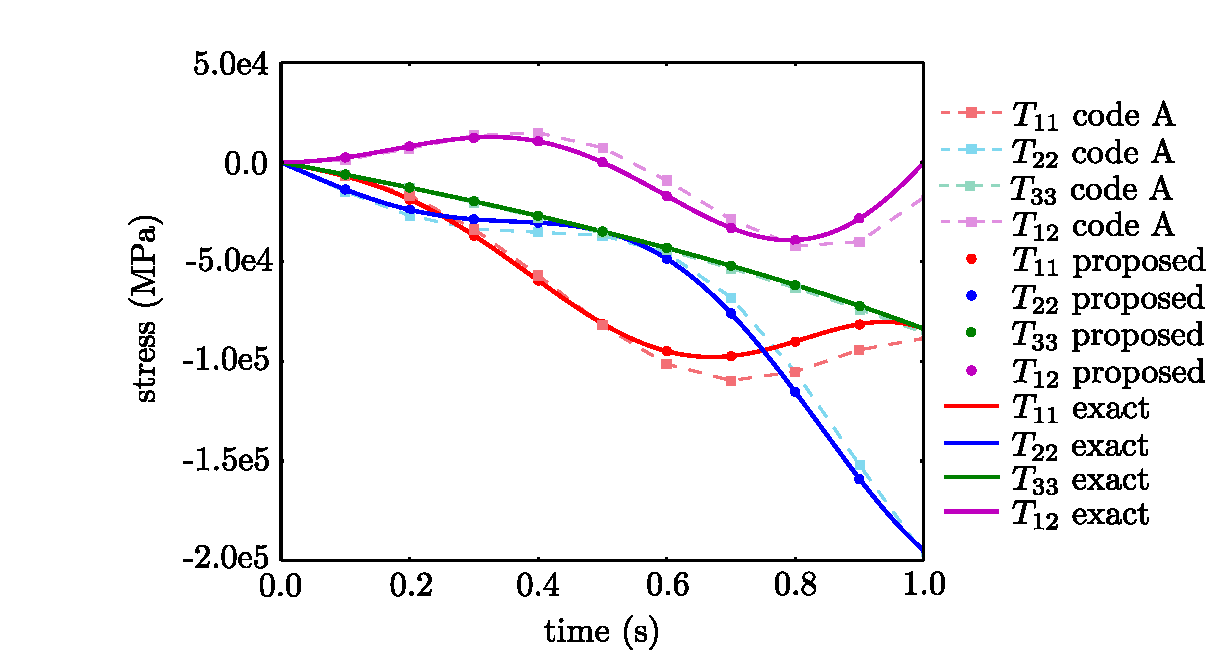
\includegraphics[scale=0.75]{src/media/stretch_rotate}
% where an .eps filename suffix will be assumed under latex,
% and a .pdf suffix will be assumed for pdflatex
\caption{Stress components plotted vs. time for the problem of uniaxial compression with finite rotation.}
\label{fig.v1-cm1}
\end{figure}

Worst-case relative errors between the exact solution $\mathbf{T}$ and approximate solutions $\mathbf{T}^h$ were computed via
\begin{equation}
    \text{\% error } (\mathbf{T}^h) = \sqrt{\frac{\max_{t} (\mathbf{T}^h - \mathbf{T}) \colon (\mathbf{T}^h - \mathbf{T})}{\max_{t} \mathbf{T} \colon \mathbf{T}}} \times 100 \% ,
    \label{eq:relative_error}
\end{equation}
and tabulated in table \ref{tab.v1-cm1}.

\begin{table}[]
\centering
\caption{Relative errors for the problem of uniaxial compression with finite rotation}
\label{tab.v1-cm1}
\begin{tabular}{c|c|c|c}
& code A & Rashid (1993) & proposed algorithm  \\ \hline
\% error $(\mathbf{T}^h)$ & 11.21704 & 0.01718 & 0.00014
\end{tabular}
\end{table}

%%%%%%%%%%%%%%%%%%%%%%%%%%%%%%%%%%%%%%%%%%%%%%%
%%%%%%%%%%%%%%%%%%%%%%%%%%%%%%%%%%%%%%%%%%%%%%%
\FloatBarrier
\subsection{Cyclic Shear}
%
In a retrospective examination of solution accuracy, the problem discussed in \cite{rashid1996} will be examined within the present context. The problem consists of a block of material which is subjected to a simple, cyclic shearing deformation given by
\begin{equation}
    \mathbf{F} = \left[ \begin{array}{ccc} 1 & \gamma & 0 \\ 0 & 1 & 0 \\ 0 & 0 & 1 \end{array} \right], \qquad \mathbf{L} = \left[ \begin{array}{ccc} 0 & \dot{\gamma} & 0 \\ 0 & 0 & 0 \\ 0 & 0 & 0 \end{array} \right],
\end{equation}
and where
\begin{equation}
    \gamma (t) = 2 \Gamma \bigg( \frac{2t}{T} - \left\lfloor \frac{2t}{T} + \frac{1}{2} \right\rfloor \bigg) (-1)^{\left\lfloor \frac{2t}{T} + \frac{1}{2} \right\rfloor}
\end{equation}
corresponds to the triangle wave with period $T$ and peak amplitude $\Gamma$, whose time derivative
\begin{equation}
    \dot{\gamma} (t) = \frac{4 \Gamma}{T} (-1)^{\left\lfloor \frac{2t}{T} + \frac{1}{2} \right\rfloor}
\end{equation}
is the square wave with period $T$. As before, the isotropic hypoelastic model of grade zero will be employed, where $\mu = E/2(1+\nu)$ represents the shear modulus of the material. The exact solution for the Cauchy stress components according to the Jaumann rate is given by the solution to the differential equation:
\begin{equation}
    \left\{ \begin{array}{c} \dot{T}_{11} \\ \dot{T}_{22} \\ \dot{T}_{12} \end{array} \right\} = \left[ \begin{array}{ccc} 0 & 0 & \dot{\gamma} \\ 0 & 0 & - \dot{\gamma} \\ -\dot{\gamma}/2 & \dot{\gamma}/2 & 0 \end{array} \right] \left\{ \begin{array}{c} T_{11} \\ T_{22} \\ T_{12} \end{array} \right\} + \mu \left\{ \begin{array}{c} 0 \\ 0 \\ \dot{\gamma} \end{array} \right\},
\end{equation}
which yields
\begin{equation}
    \left\{ \begin{array}{c} T_{11} \\ T_{22} \\ T_{33} \\ T_{23} \\ T_{13} \\ T_{12} \end{array} \right\} = \left\{ \begin{array}{c} \mu (1-\cos \gamma (t)) \\ \mu (\cos \gamma (t) - 1) \\ 0 \\ 0 \\ 0 \\ \mu \sin \gamma (t) \end{array} \right\}.
\end{equation}
Numerical solutions were computed for the values $\Gamma = 0.5$, $E = 2.09 \times 10^5$, $\nu = 0.3$, $T = 1.0$, and $t \in \left[ 0, 2 \right]$, yielding 2 complete cycles of deformation. The results are depicted in figure \ref{fig.cyclic_shear-cm1}.

\begin{figure}
\centering
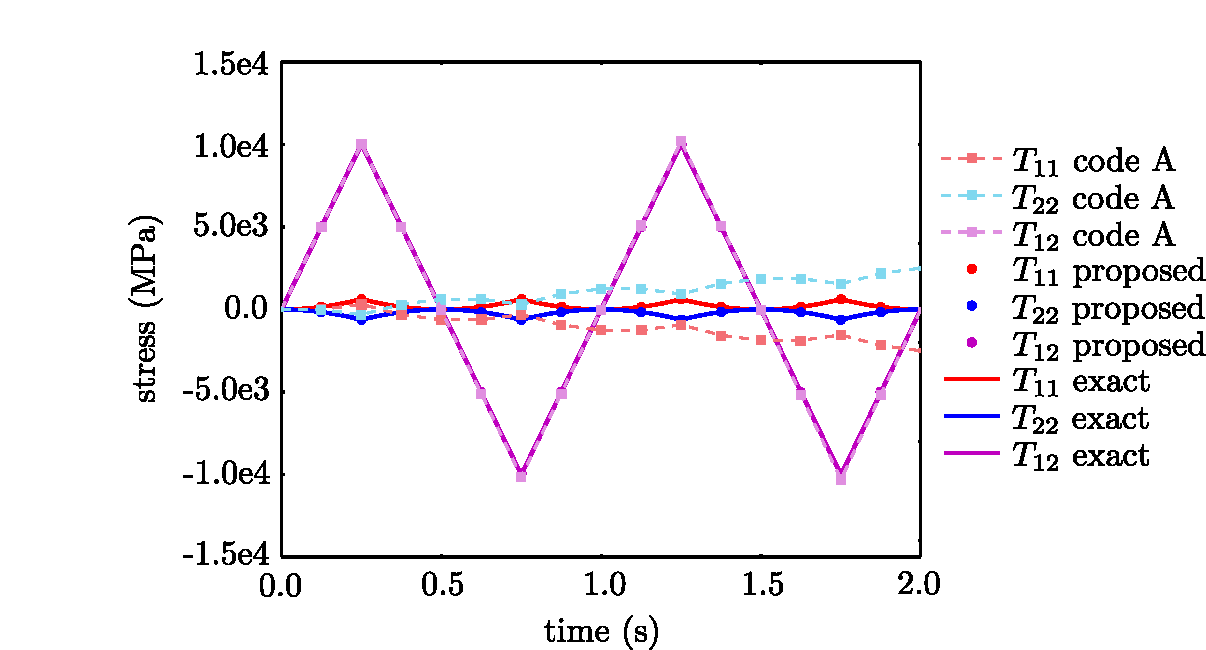
\includegraphics[scale=0.75]{src/media/cyclic_shear}
% where an .eps filename suffix will be assumed under latex,
% and a .pdf suffix will be assumed for pdflatex
\caption{Stress components plotted vs. time for the problem of cyclic shear.}
\label{fig.cyclic_shear-cm1}
\end{figure}

Worst-case relative errors between the exact solution $\mathbf{T}$ and approximate solutions $\mathbf{T}^h$ were computed via equation \ref{eq:relative_error} and tabulated in table \ref{tab.cyclic_shear-cm1}.

\begin{table}[]
\centering
\caption{Relative errors for the problem of cyclic shear}
\label{tab.cyclic_shear-cm1}
\begin{tabular}{c|c|c|c}
& code A & Rashid (1993) & proposed algorithm  \\ \hline
\% error $(\mathbf{T}^h)$ & 24.94638 & 0.00227 & 0.00205
\end{tabular}
\end{table}

%%%%%%%%%%%%%%%%%%%%%%%%%%%%%%%%%%%%%%%%%%%%%%%
%%%%%%%%%%%%%%%%%%%%%%%%%%%%%%%%%%%%%%%%%%%%%%%
\FloatBarrier
\subsection{Twisting Prism}

\begin{figure}[!tbhp]
\centering
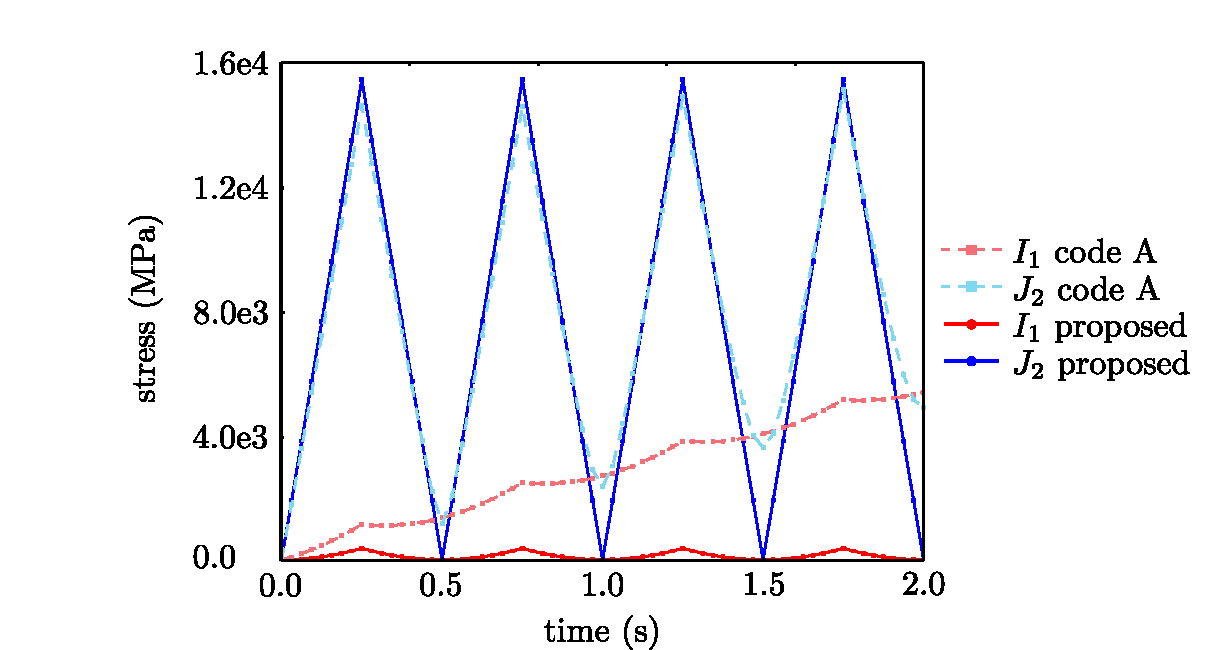
\includegraphics[scale=0.75]{media/twisted_prism}
% where an .eps filename suffix will be assumed under latex,
% and a .pdf suffix will be assumed for pdflatex
\caption{Stress measures plotted vs. time for the twisting prism problem, where $I_1$ is the first invariant of the Cauchy stress tensor, and $J_2$ is the second invariant of the deviatoric stress tensor}
\label{fig.twisted_prism-cm1}
\end{figure}
\negparafig

%%%%%%%%%%%%%%%%%%%%%%%%%%%%%%%%%%%%%%%%%%%%%%%
%%%%%%%%%%%%%%%%%%%%%%%%%%%%%%%%%%%%%%%%%%%%%%%
\section{Performance Evaluation of Nonlinear Solution Convergence}
%

\begin{figure}[!tbhp]
\centering
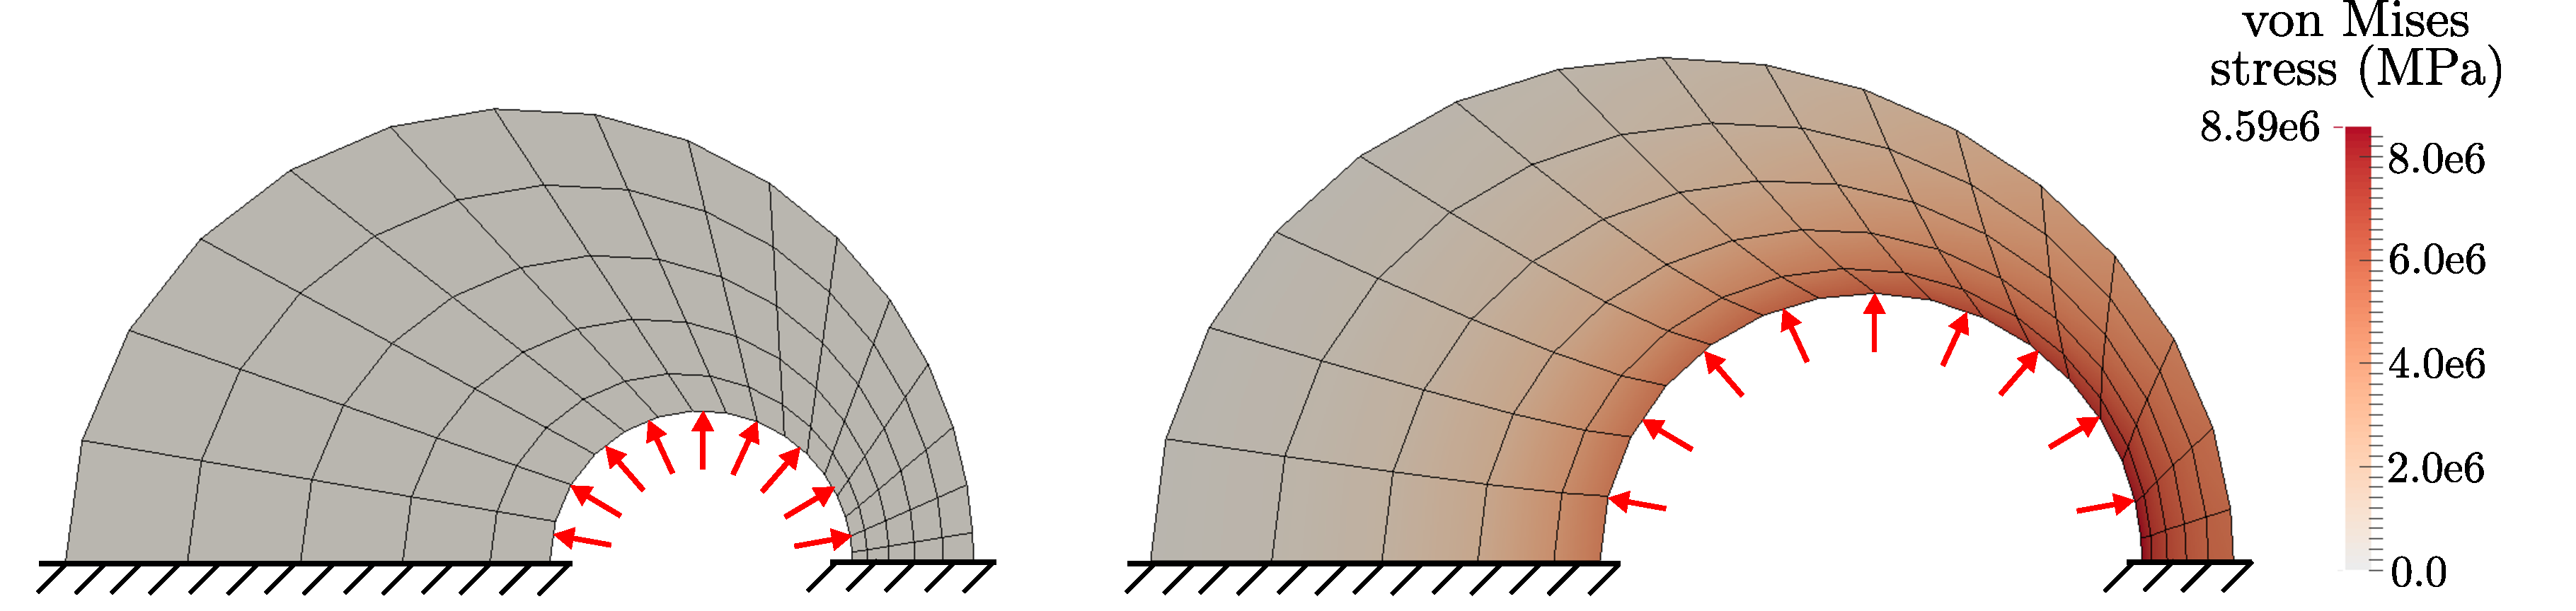
\includegraphics[scale=0.28]{media/ring_problem}
% where an .eps filename suffix will be assumed under latex,
% and a .pdf suffix will be assumed for pdflatex
\caption{Pressurized eccentric cylinder modeled with half-symmetry.}
\label{fig.ring}
\end{figure}

\begin{table}[]
\centering
\caption{Number of Newton-Raphson iterations per time step for the eccentric cylinder problem}
\label{tab.ring}
\begin{tabular}{|c|c|c|c|}
\hline
Step & Hughes-Winget & Rashid (1993) & Proposed Algorithm  \\ \hline
1  & 3 & 3  & 3 \\ \hline
2  & 2 & 2  & 2 \\ \hline
3  & 2 & 2  & 2 \\ \hline
4  & 2 & 2  & 2 \\ \hline
5  & 2 & 2  & 2 \\ \hline
6  & 2 & 3  & 2 \\ \hline
7  & 2 & 3  & 2 \\ \hline
8  & 2 & 3  & 2 \\ \hline
9  & 3 & 4  & 3 \\ \hline
10 & 4 & 27 & 4\\ \hline
\end{tabular}
\end{table}

\begin{table}[]
\centering
\caption{Number of Newton-Raphson iterations using an inconsistent linearization}
\label{tab.ring_tangents}
\begin{tabular}{|c|c|c|c|c|}
\hline
Step & Consistent & Rotation Off & Pressure Off & Rotation \& Pressure Off \\ \hline
1  & 3 & 5   & 6  & 6 \\ \hline
2  & 2 & 5   & 7  & 8 \\ \hline
3  & 2 & 6   & 9  & 10 \\ \hline
4  & 2 & 6   & 11 & 13 \\ \hline
5  & 2 & 8   & 14 & 16 \\ \hline
6  & 2 & 10  & 18 & 20 \\ \hline
7  & 2 & 14  & 25 & 24 \\ \hline
8  & 2 & 22  & 42 & 31 \\ \hline
9  & 3 & 40  & 123 & 41 \\ \hline
10 & 4 & 771 & $>$1000 & 784 \\ \hline
\end{tabular}
\end{table}
\section{Conclusions}
%
\section{Appendix}
%


%%%%%%%%%%%%%%%%%%%%%%%%%%%%%%%%%%%%%%%%%%%%%%%%%%%%%%%%%%%%%%%%%%%%%%%%

\bibliography{references}

%%%%%%%%%%%%%%%%%%%%%%%%%%%%%%%%%%%%%%%%%%%%%%%%%%%%%%%%%%%%%%%%%%%%%%%%

\end{document}